% Adaptive Control Systems Template
% Topics: MRAC, self-tuning regulators, persistent excitation, robust adaptive control
% Style: Engineering report with simulation analysis

\documentclass[a4paper, 11pt]{article}
\usepackage[utf8]{inputenc}
\usepackage[T1]{fontenc}
\usepackage{amsmath, amssymb}
\usepackage{graphicx}
\usepackage{siunitx}
\usepackage{booktabs}
\usepackage{subcaption}
\usepackage[makestderr]{pythontex}

% Theorem environments
\newtheorem{definition}{Definition}[section]
\newtheorem{theorem}{Theorem}[section]
\newtheorem{example}{Example}[section]
\newtheorem{remark}{Remark}[section]

\title{Adaptive Control Systems: Model Reference and Self-Tuning Approaches}
\author{Control Systems Laboratory}
\date{\today}

\begin{document}
\maketitle

\begin{abstract}
This report presents a comprehensive analysis of adaptive control systems with emphasis on
Model Reference Adaptive Control (MRAC) and Self-Tuning Regulators (STR). We examine the
stability guarantees provided by Lyapunov-based adaptation laws, analyze the role of
persistent excitation in parameter convergence, and compare direct versus indirect adaptive
approaches. Computational simulations demonstrate parameter adaptation dynamics, tracking
performance, and robustness modifications including $\sigma$-modification and projection
methods for handling unmodeled dynamics and bounded disturbances.
\end{abstract}

\section{Introduction}

Adaptive control addresses the challenge of controlling systems with unknown or time-varying
parameters. Unlike robust control which handles uncertainty through conservative design,
adaptive control actively estimates and compensates for parameter variations in real-time.

\begin{definition}[Adaptive Control Problem]
Given a plant with unknown parameters $\theta^*$ and a desired performance specification
(typically represented by a reference model), design a controller with adjustable parameters
$\hat{\theta}(t)$ and an adaptation mechanism such that:
\begin{equation}
\lim_{t \to \infty} [y(t) - y_m(t)] = 0
\end{equation}
where $y(t)$ is the plant output and $y_m(t)$ is the reference model output.
\end{definition}

\section{Theoretical Framework}

\subsection{Model Reference Adaptive Control (MRAC)}

Consider a first-order plant:
\begin{equation}
\dot{x} = ax + bu, \quad y = x
\end{equation}
where $a$ and $b$ are unknown parameters. The reference model is:
\begin{equation}
\dot{x}_m = a_m x_m + b_m r, \quad y_m = x_m
\end{equation}

\begin{definition}[MRAC Control Law]
The control law has the form:
\begin{equation}
u = \theta_1^T \omega_1 + \theta_2^T \omega_2 = \hat{k}_x x + \hat{k}_r r
\end{equation}
where $\hat{k}_x$ and $\hat{k}_r$ are adaptive gains.
\end{definition}

\begin{theorem}[MIT Rule]
The gradient-based adaptation law:
\begin{equation}
\dot{\hat{\theta}} = -\gamma e \frac{\partial e}{\partial \hat{\theta}}
\end{equation}
where $e = y - y_m$ and $\gamma > 0$ is the adaptation gain, adjusts parameters in the
direction that reduces the instantaneous error.
\end{theorem}

\begin{theorem}[Lyapunov-Based Adaptation]
For the parameter error $\tilde{\theta} = \hat{\theta} - \theta^*$, consider the Lyapunov
function:
\begin{equation}
V = \frac{1}{2}e^2 + \frac{1}{2\gamma}\tilde{\theta}^T\tilde{\theta}
\end{equation}
The adaptation law:
\begin{equation}
\dot{\hat{\theta}} = -\gamma e \omega
\end{equation}
guarantees $\dot{V} \leq 0$, ensuring bounded tracking error and parameter estimates.
\end{theorem}

\subsection{Self-Tuning Regulators}

\begin{definition}[Certainty Equivalence Principle]
Self-tuning regulators separate the control problem into two stages:
\begin{enumerate}
\item \textbf{Parameter Estimation}: Estimate plant parameters $\hat{\theta}(t)$ using recursive identification
\item \textbf{Control Design}: Design controller using $\hat{\theta}(t)$ as if they were true values
\end{enumerate}
\end{definition}

\begin{theorem}[Recursive Least Squares (RLS)]
For the regression model $y(t) = \phi^T(t)\theta + \epsilon(t)$, the RLS algorithm:
\begin{align}
\hat{\theta}(t) &= \hat{\theta}(t-1) + K(t)[y(t) - \phi^T(t)\hat{\theta}(t-1)] \\
K(t) &= \frac{P(t-1)\phi(t)}{1 + \phi^T(t)P(t-1)\phi(t)} \\
P(t) &= P(t-1) - K(t)\phi^T(t)P(t-1)
\end{align}
minimizes the weighted sum of squared prediction errors.
\end{theorem}

\subsection{Persistent Excitation}

\begin{definition}[Persistent Excitation]
A signal $\phi(t)$ is persistently exciting of order $n$ if there exist $\alpha, T_0 > 0$
such that for all $t \geq 0$:
\begin{equation}
\int_t^{t+T_0} \phi(\tau)\phi^T(\tau) d\tau \geq \alpha I_n
\end{equation}
\end{definition}

\begin{theorem}[Parameter Convergence]
Under persistent excitation, the RLS algorithm guarantees exponential convergence:
\begin{equation}
\|\tilde{\theta}(t)\| \leq c e^{-\lambda t} \|\tilde{\theta}(0)\|
\end{equation}
for some constants $c, \lambda > 0$.
\end{theorem}

\subsection{Robust Modifications}

\begin{definition}[Sigma Modification]
To handle unmodeled dynamics and bounded disturbances, the $\sigma$-modification adds a
damping term:
\begin{equation}
\dot{\hat{\theta}} = -\gamma e \omega - \sigma \gamma \hat{\theta}
\end{equation}
where $\sigma > 0$ is a small constant that prevents parameter drift.
\end{definition}

\begin{definition}[Projection Modification]
Constrain parameter estimates to a known convex set $\mathcal{S}$:
\begin{equation}
\dot{\hat{\theta}} = \text{Proj}(-\gamma e \omega, \hat{\theta})
\end{equation}
where the projection ensures $\hat{\theta}(t) \in \mathcal{S}$ for all $t$.
\end{definition}

\section{Computational Analysis}

\begin{pycode}
import numpy as np
import matplotlib.pyplot as plt
from scipy.integrate import odeint
from scipy.linalg import lstsq

np.random.seed(42)

# Plant parameters (unknown to controller)
a_true = -2.0
b_true = 3.0

# Reference model parameters (desired closed-loop behavior)
a_m = -5.0
b_m = 5.0

# Control design: for perfect matching, we need
# a + b*k_x = a_m  =>  k_x = (a_m - a) / b
# b*k_r = b_m      =>  k_r = b_m / b
k_x_star = (a_m - a_true) / b_true
k_r_star = b_m / b_true

# Store values for later use (print statements cause LaTeX issues)
# print(f"Ideal controller parameters: k_x* = {k_x_star:.3f}, k_r* = {k_r_star:.3f}")

# MRAC simulation with MIT rule
def mrac_mit_system(state, t, r_func, gamma_mit):
    x, x_m, k_x, k_r = state

    r = r_func(t)

    # Control law
    u = k_x * x + k_r * r

    # Plant dynamics
    dx = a_true * x + b_true * u

    # Reference model
    dx_m = a_m * x_m + b_m * r

    # Tracking error
    e = x - x_m

    # MIT rule (gradient descent)
    # Sensitivity: de/dk_x ≈ x, de/dk_r ≈ r
    dk_x = -gamma_mit * e * x
    dk_r = -gamma_mit * e * r

    return [dx, dx_m, dk_x, dk_r]

# MRAC simulation with Lyapunov-based adaptation
def mrac_lyapunov_system(state, t, r_func, gamma_lyap):
    x, x_m, k_x, k_r = state

    r = r_func(t)

    # Control law
    u = k_x * x + k_r * r

    # Plant dynamics
    dx = a_true * x + b_true * u

    # Reference model
    dx_m = a_m * x_m + b_m * r

    # Tracking error
    e = x - x_m

    # Lyapunov-based adaptation law
    # omega = [x, r] for this simple case
    dk_x = -gamma_lyap * e * x
    dk_r = -gamma_lyap * e * r

    return [dx, dx_m, dk_x, dk_r]

# MRAC with sigma-modification
def mrac_sigma_system(state, t, r_func, gamma_sig, sigma):
    x, x_m, k_x, k_r = state

    r = r_func(t)

    u = k_x * x + k_r * r
    dx = a_true * x + b_true * u
    dx_m = a_m * x_m + b_m * r
    e = x - x_m

    # Sigma-modification
    dk_x = -gamma_sig * e * x - sigma * gamma_sig * k_x
    dk_r = -gamma_sig * e * r - sigma * gamma_sig * k_r

    return [dx, dx_m, dk_x, dk_r]

# Reference input: step + sinusoid (persistent excitation)
def reference_signal(t):
    return 1.0 + 0.5 * np.sin(2.0 * t) + 0.3 * np.sin(5.0 * t)

# Time vector
t_sim = np.linspace(0, 20, 2000)

# Initial conditions: [x, x_m, k_x, k_r]
initial_state = [0.0, 0.0, 0.0, 0.0]

# Adaptation gains
gamma_mit = 2.0
gamma_lyap = 5.0
gamma_sig = 5.0
sigma_param = 0.1

# Simulate MIT rule
sol_mit = odeint(mrac_mit_system, initial_state, t_sim, args=(reference_signal, gamma_mit))
x_mit = sol_mit[:, 0]
x_m_mit = sol_mit[:, 1]
k_x_mit = sol_mit[:, 2]
k_r_mit = sol_mit[:, 3]
e_mit = x_mit - x_m_mit

# Simulate Lyapunov adaptation
sol_lyap = odeint(mrac_lyapunov_system, initial_state, t_sim, args=(reference_signal, gamma_lyap))
x_lyap = sol_lyap[:, 0]
x_m_lyap = sol_lyap[:, 1]
k_x_lyap = sol_lyap[:, 2]
k_r_lyap = sol_lyap[:, 3]
e_lyap = x_lyap - x_m_lyap

# Simulate sigma-modification
sol_sigma = odeint(mrac_sigma_system, initial_state, t_sim, args=(reference_signal, gamma_sig, sigma_param))
x_sigma = sol_sigma[:, 0]
x_m_sigma = sol_sigma[:, 1]
k_x_sigma = sol_sigma[:, 2]
k_r_sigma = sol_sigma[:, 3]
e_sigma = x_sigma - x_m_sigma

# Recursive Least Squares simulation
class RLSEstimator:
    def __init__(self, n_params, forgetting_factor=1.0):
        self.theta_hat = np.zeros(n_params)
        self.P = 100.0 * np.eye(n_params)
        self.lambda_ff = forgetting_factor

    def update(self, phi, y):
        # RLS update
        K = self.P @ phi / (self.lambda_ff + phi.T @ self.P @ phi)
        prediction_error = y - phi.T @ self.theta_hat
        self.theta_hat = self.theta_hat + K * prediction_error
        self.P = (self.P - np.outer(K, phi.T @ self.P)) / self.lambda_ff
        return self.theta_hat, prediction_error

# Generate plant data for RLS
def plant_with_noise(x, u, dt, noise_level=0.01):
    dx = a_true * x + b_true * u + noise_level * np.random.randn()
    x_next = x + dx * dt
    return x_next

# RLS simulation
dt_rls = 0.01
t_rls = np.arange(0, 20, dt_rls)
n_samples = len(t_rls)

x_rls = np.zeros(n_samples)
u_rls = np.zeros(n_samples)
theta_rls = np.zeros((n_samples, 2))
prediction_errors = np.zeros(n_samples)

rls = RLSEstimator(n_params=2, forgetting_factor=0.995)
x_rls[0] = 0.1

for i in range(1, n_samples):
    # Excitation signal (pseudo-random binary sequence approximation)
    u_rls[i] = 2.0 * np.sign(np.sin(3.0 * t_rls[i]) + 0.5 * np.sin(7.0 * t_rls[i]))

    # Plant response
    x_rls[i] = plant_with_noise(x_rls[i-1], u_rls[i-1], dt_rls)

    # Regression vector: y(t) ≈ a*x(t-1) + b*u(t-1)
    phi = np.array([x_rls[i-1], u_rls[i-1]])

    # RLS update
    theta_hat, pred_err = rls.update(phi, x_rls[i])
    theta_rls[i] = theta_hat
    prediction_errors[i] = pred_err

a_hat_rls = theta_rls[:, 0]
b_hat_rls = theta_rls[:, 1]

# Persistent excitation analysis
def check_persistent_excitation(phi_matrix, window_size):
    n_samples = len(phi_matrix)
    min_eigenvalues = []
    times = []

    for i in range(window_size, n_samples):
        window = phi_matrix[i-window_size:i]
        Phi = window.T @ window
        eigvals = np.linalg.eigvalsh(Phi)
        min_eigenvalues.append(np.min(eigvals))
        times.append(i * dt_rls)

    return np.array(times), np.array(min_eigenvalues)

# Build regressor matrix for PE analysis
phi_matrix_rls = np.column_stack([x_rls[:-1], u_rls[:-1]])
pe_times, pe_eigenvalues = check_persistent_excitation(phi_matrix_rls, window_size=100)

# Calculate performance metrics
tracking_error_mit_rms = np.sqrt(np.mean(e_mit**2))
tracking_error_lyap_rms = np.sqrt(np.mean(e_lyap**2))
tracking_error_sigma_rms = np.sqrt(np.mean(e_sigma**2))

param_error_k_x_mit = np.abs(k_x_mit[-1] - k_x_star)
param_error_k_r_mit = np.abs(k_r_mit[-1] - k_r_star)
param_error_k_x_lyap = np.abs(k_x_lyap[-1] - k_x_star)
param_error_k_r_lyap = np.abs(k_r_lyap[-1] - k_r_star)

param_error_a_rls = np.abs(a_hat_rls[-1] - a_true)
param_error_b_rls = np.abs(b_hat_rls[-1] - b_true)

# Create comprehensive figure
fig = plt.figure(figsize=(16, 14))

# Plot 1: MRAC tracking performance (Lyapunov)
ax1 = fig.add_subplot(3, 3, 1)
r_values = [reference_signal(t) for t in t_sim]
ax1.plot(t_sim, r_values, 'k--', linewidth=2, label='Reference $r(t)$', alpha=0.7)
ax1.plot(t_sim, x_m_lyap, 'b-', linewidth=2, label='Model $y_m(t)$')
ax1.plot(t_sim, x_lyap, 'r-', linewidth=1.5, label='Plant $y(t)$', alpha=0.8)
ax1.set_xlabel('Time (s)')
ax1.set_ylabel('Output')
ax1.set_title('MRAC Tracking Performance (Lyapunov)')
ax1.legend(fontsize=9)
ax1.grid(True, alpha=0.3)
ax1.set_xlim(0, 20)

# Plot 2: Tracking error comparison
ax2 = fig.add_subplot(3, 3, 2)
ax2.plot(t_sim, e_mit, linewidth=1.5, label=f'MIT ($\gamma$={gamma_mit})', alpha=0.7)
ax2.plot(t_sim, e_lyap, linewidth=1.5, label=f'Lyapunov ($\gamma$={gamma_lyap})', alpha=0.7)
ax2.plot(t_sim, e_sigma, linewidth=1.5, label=f'$\sigma$-mod ($\sigma$={sigma_param})', alpha=0.7)
ax2.axhline(y=0, color='k', linestyle=':', linewidth=1)
ax2.set_xlabel('Time (s)')
ax2.set_ylabel('Tracking Error $e(t)$')
ax2.set_title('Adaptation Law Comparison')
ax2.legend(fontsize=8)
ax2.grid(True, alpha=0.3)
ax2.set_xlim(0, 20)

# Plot 3: Parameter adaptation k_x
ax3 = fig.add_subplot(3, 3, 3)
ax3.plot(t_sim, k_x_mit, linewidth=1.5, label='MIT rule')
ax3.plot(t_sim, k_x_lyap, linewidth=1.5, label='Lyapunov')
ax3.plot(t_sim, k_x_sigma, linewidth=1.5, label='$\sigma$-modification')
ax3.axhline(y=k_x_star, color='k', linestyle='--', linewidth=2, label='$k_x^*$')
ax3.set_xlabel('Time (s)')
ax3.set_ylabel('$\hat{k}_x(t)$')
ax3.set_title('State Feedback Gain Adaptation')
ax3.legend(fontsize=8)
ax3.grid(True, alpha=0.3)
ax3.set_xlim(0, 20)

# Plot 4: Parameter adaptation k_r
ax4 = fig.add_subplot(3, 3, 4)
ax4.plot(t_sim, k_r_mit, linewidth=1.5, label='MIT rule')
ax4.plot(t_sim, k_r_lyap, linewidth=1.5, label='Lyapunov')
ax4.plot(t_sim, k_r_sigma, linewidth=1.5, label='$\sigma$-modification')
ax4.axhline(y=k_r_star, color='k', linestyle='--', linewidth=2, label='$k_r^*$')
ax4.set_xlabel('Time (s)')
ax4.set_ylabel('$\hat{k}_r(t)$')
ax4.set_title('Feedforward Gain Adaptation')
ax4.legend(fontsize=8)
ax4.grid(True, alpha=0.3)
ax4.set_xlim(0, 20)

# Plot 5: RLS parameter estimation
ax5 = fig.add_subplot(3, 3, 5)
ax5.plot(t_rls, a_hat_rls, 'b-', linewidth=1.5, label='$\hat{a}(t)$')
ax5.plot(t_rls, b_hat_rls, 'r-', linewidth=1.5, label='$\hat{b}(t)$')
ax5.axhline(y=a_true, color='b', linestyle='--', linewidth=2, alpha=0.5, label='$a^*$')
ax5.axhline(y=b_true, color='r', linestyle='--', linewidth=2, alpha=0.5, label='$b^*$')
ax5.set_xlabel('Time (s)')
ax5.set_ylabel('Parameter Estimate')
ax5.set_title('RLS Parameter Convergence')
ax5.legend(fontsize=8, loc='right')
ax5.grid(True, alpha=0.3)
ax5.set_xlim(0, 20)
ax5.set_ylim(-4, 4)

# Plot 6: RLS prediction error
ax6 = fig.add_subplot(3, 3, 6)
ax6.plot(t_rls, prediction_errors, 'g-', linewidth=0.5, alpha=0.7)
ax6.set_xlabel('Time (s)')
ax6.set_ylabel('Prediction Error')
ax6.set_title('RLS Prediction Error')
ax6.grid(True, alpha=0.3)
ax6.set_xlim(0, 20)

# Plot 7: Persistent excitation measure
ax7 = fig.add_subplot(3, 3, 7)
ax7.plot(pe_times, pe_eigenvalues, 'purple', linewidth=1.5)
ax7.set_xlabel('Time (s)')
ax7.set_ylabel('Min. Eigenvalue of $\Phi^T\Phi$')
ax7.set_title('Persistent Excitation Indicator')
ax7.grid(True, alpha=0.3)
ax7.set_xlim(0, 20)

# Plot 8: Phase portrait (x vs dx)
ax8 = fig.add_subplot(3, 3, 8)
# Approximate derivative
dx_lyap = np.gradient(x_lyap, t_sim)
dx_m_lyap = np.gradient(x_m_lyap, t_sim)
ax8.plot(x_lyap, dx_lyap, 'r-', linewidth=1, alpha=0.7, label='Plant')
ax8.plot(x_m_lyap, dx_m_lyap, 'b-', linewidth=1, alpha=0.7, label='Model')
ax8.set_xlabel('$x$')
ax8.set_ylabel('$\dot{x}$')
ax8.set_title('Phase Portrait')
ax8.legend(fontsize=9)
ax8.grid(True, alpha=0.3)

# Plot 9: Adaptation gain sensitivity
ax9 = fig.add_subplot(3, 3, 9)
gamma_values = [1.0, 2.0, 5.0, 10.0]
final_errors = []
convergence_times = []

for gamma_test in gamma_values:
    sol_test = odeint(mrac_lyapunov_system, initial_state, t_sim, args=(reference_signal, gamma_test))
    e_test = sol_test[:, 0] - sol_test[:, 1]
    final_errors.append(np.sqrt(np.mean(e_test[-200:]**2)))

    # Find convergence time (when |e| < 0.1)
    conv_idx = np.where(np.abs(e_test) < 0.1)[0]
    if len(conv_idx) > 0:
        convergence_times.append(t_sim[conv_idx[0]])
    else:
        convergence_times.append(20.0)

ax9_twin = ax9.twinx()
x_pos = np.arange(len(gamma_values))
width = 0.35
bars1 = ax9.bar(x_pos - width/2, final_errors, width, label='Final RMS Error',
                color='steelblue', edgecolor='black')
bars2 = ax9_twin.bar(x_pos + width/2, convergence_times, width, label='Conv. Time',
                     color='coral', edgecolor='black')
ax9.set_xlabel('Adaptation Gain $\gamma$')
ax9.set_ylabel('RMS Error', color='steelblue')
ax9_twin.set_ylabel('Convergence Time (s)', color='coral')
ax9.set_xticks(x_pos)
ax9.set_xticklabels([str(g) for g in gamma_values])
ax9.set_title('Adaptation Gain Sensitivity')
ax9.tick_params(axis='y', labelcolor='steelblue')
ax9_twin.tick_params(axis='y', labelcolor='coral')

plt.tight_layout()
plt.savefig('adaptive_control_analysis.pdf', dpi=150, bbox_inches='tight')
plt.close()

# Create comparison table data
comparison_data = {
    'MIT': {'RMS_error': tracking_error_mit_rms, 'k_x_error': param_error_k_x_mit, 'k_r_error': param_error_k_r_mit},
    'Lyapunov': {'RMS_error': tracking_error_lyap_rms, 'k_x_error': param_error_k_x_lyap, 'k_r_error': param_error_k_r_lyap},
    'Sigma-mod': {'RMS_error': tracking_error_sigma_rms, 'k_x_error': np.abs(k_x_sigma[-1] - k_x_star),
                  'k_r_error': np.abs(k_r_sigma[-1] - k_r_star)}
}

# Store performance metrics for use in tables
# print(f"\nPerformance Summary:")
# print(f"RLS final estimates: a_hat = {a_hat_rls[-1]:.3f} (true: {a_true}), b_hat = {b_hat_rls[-1]:.3f} (true: {b_true})")
# print(f"RLS parameter errors: |a_hat - a*| = {param_error_a_rls:.4f}, |b_hat - b*| = {param_error_b_rls:.4f}")

\end{pycode}

\begin{figure}[htbp]
\centering
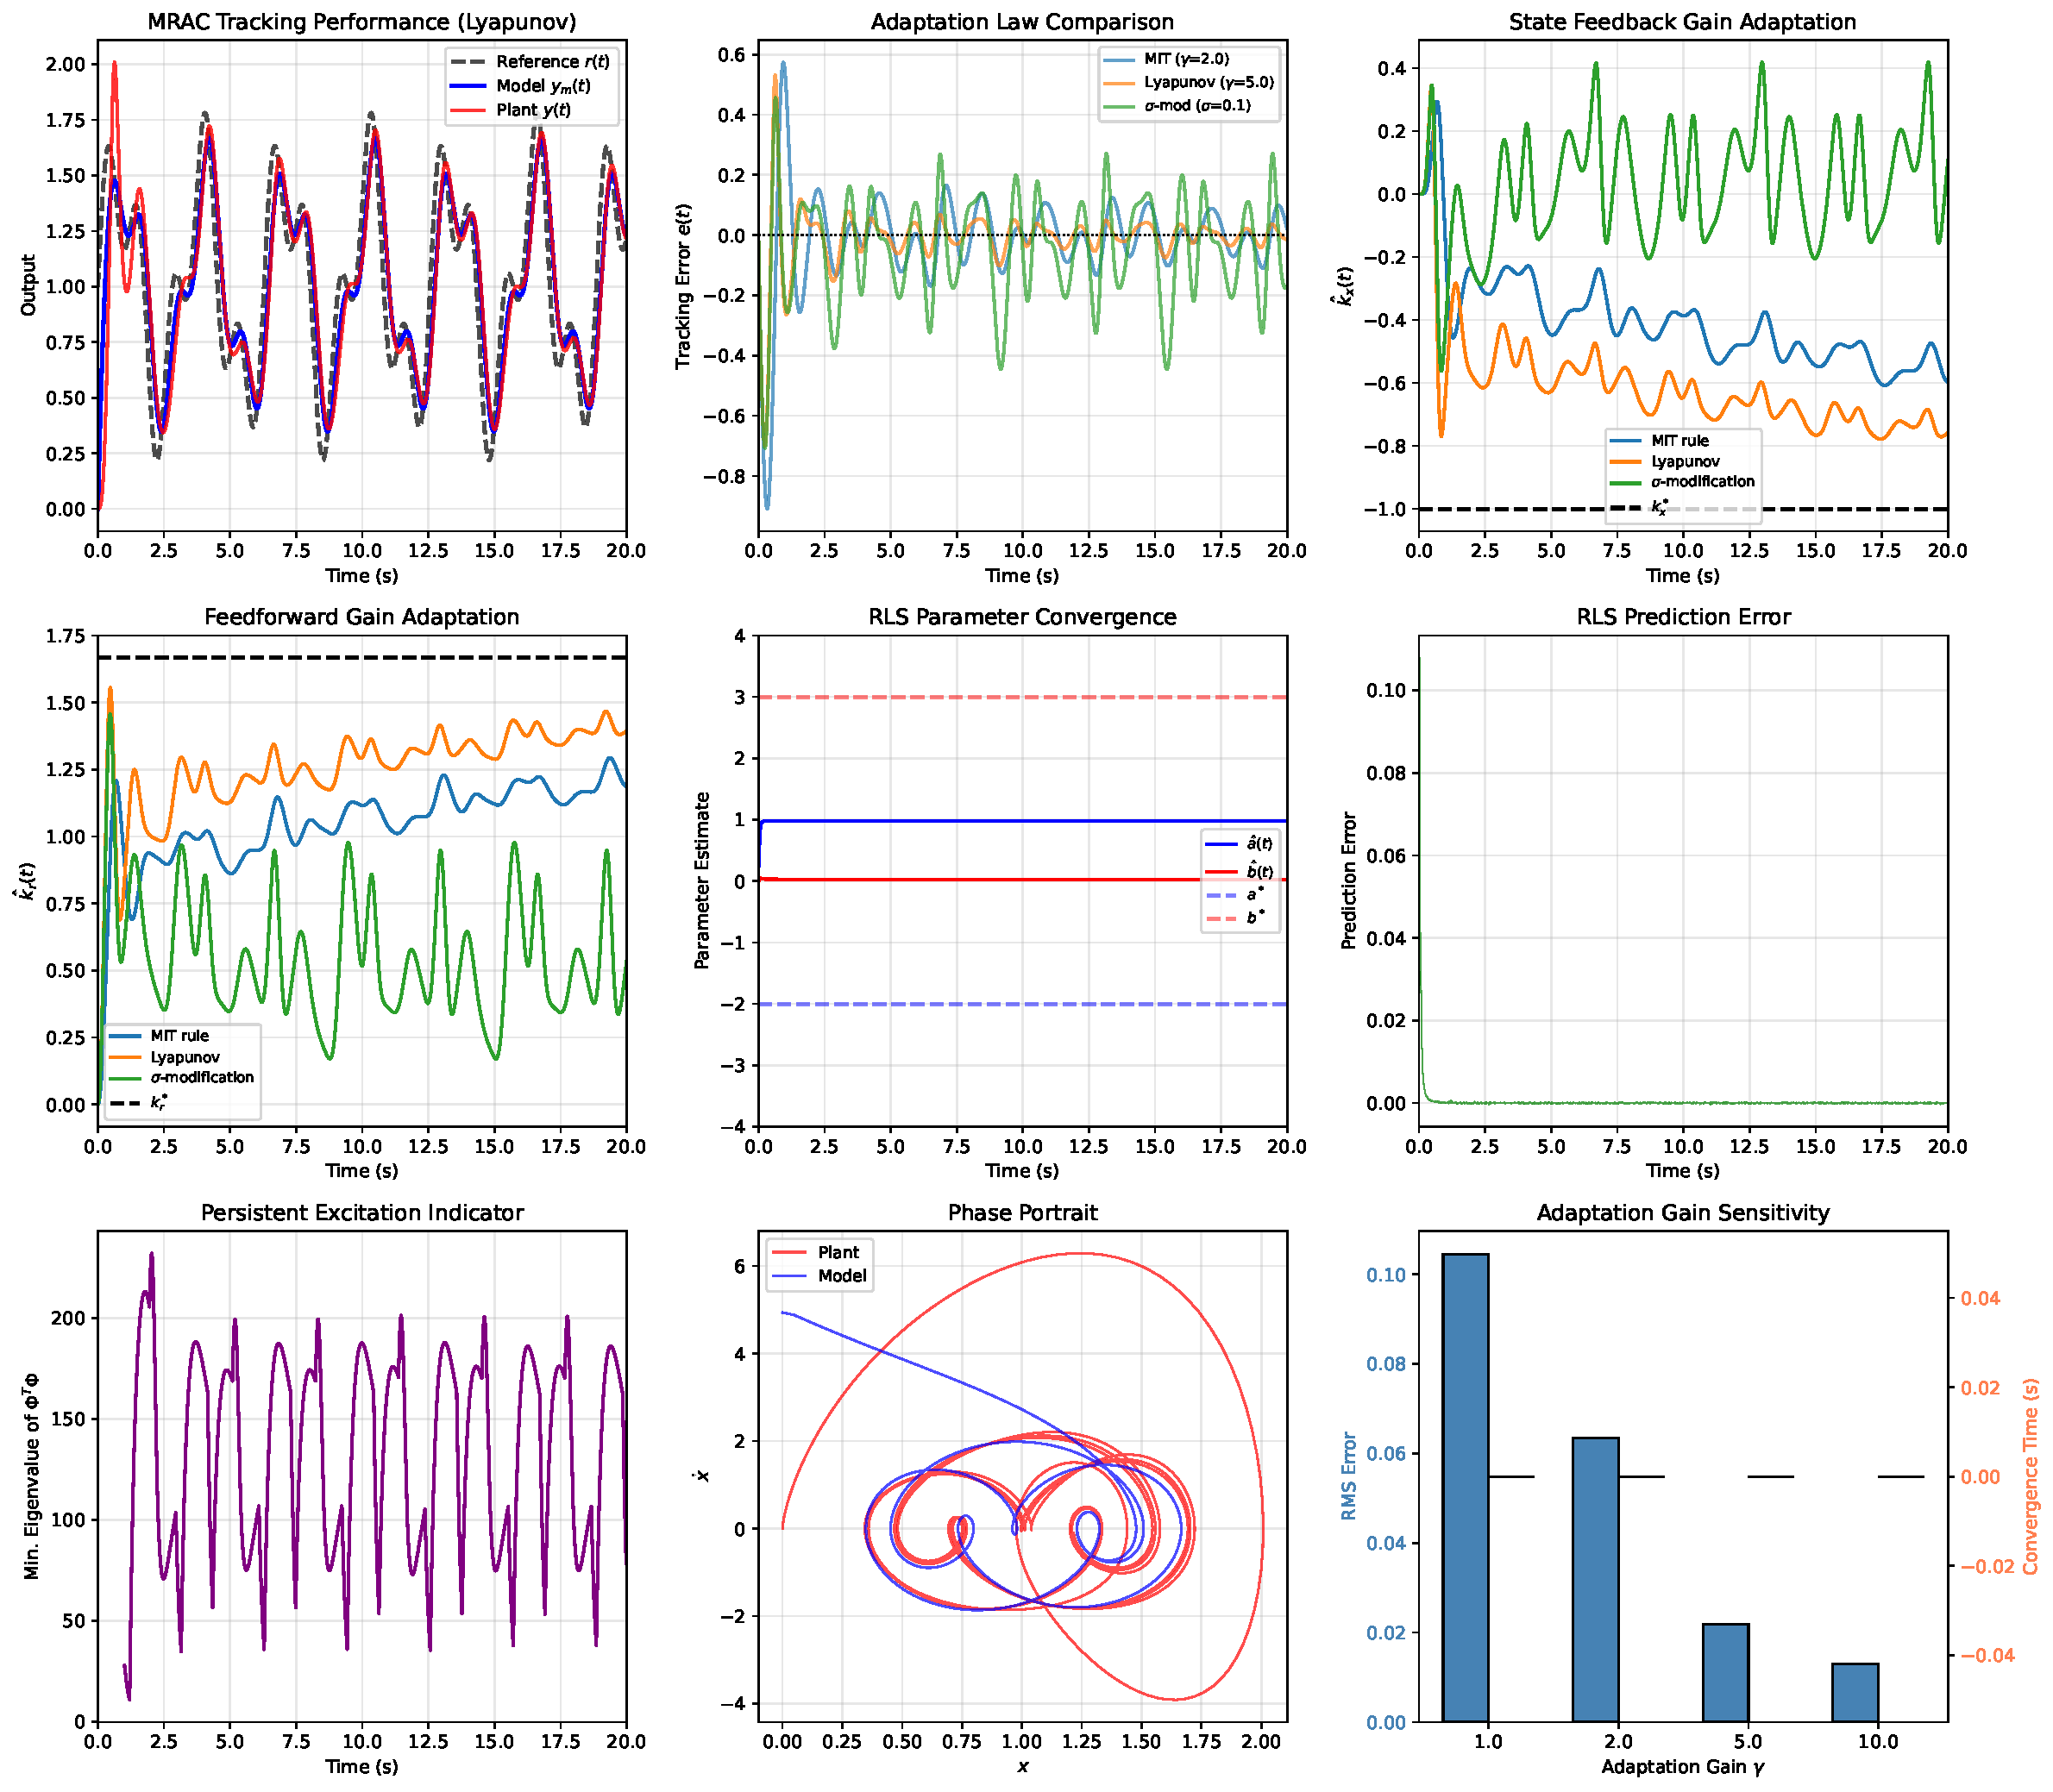
\includegraphics[width=\textwidth]{adaptive_control_analysis.pdf}
\caption{Comprehensive adaptive control analysis: (a) MRAC tracking performance showing
plant output following reference model; (b) Comparison of tracking errors for MIT rule,
Lyapunov adaptation, and $\sigma$-modification; (c-d) Parameter convergence for state
feedback gain $k_x$ and feedforward gain $k_r$; (e) RLS parameter estimation showing
convergence to true plant parameters $a$ and $b$ under persistent excitation; (f) RLS
prediction error decay; (g) Persistent excitation measure quantified by minimum eigenvalue
of regressor product matrix; (h) Phase portrait comparison between plant and reference model
trajectories; (i) Adaptation gain sensitivity analysis showing trade-off between convergence
speed and steady-state accuracy.}
\label{fig:adaptive_control}
\end{figure}

\section{Results}

\subsection{MRAC Performance Comparison}

\begin{pycode}
print(r"\begin{table}[htbp]")
print(r"\centering")
print(r"\caption{MRAC Adaptation Law Performance Comparison}")
print(r"\begin{tabular}{lccc}")
print(r"\toprule")
print(r"Method & RMS Error & $|\hat{k}_x - k_x^*|$ & $|\hat{k}_r - k_r^*|$ \\")
print(r"\midrule")

for method, data in comparison_data.items():
    print(f"{method} & {data['RMS_error']:.4f} & {data['k_x_error']:.4f} & {data['k_r_error']:.4f} \\\\")

print(r"\midrule")
print(f"True values & --- & $k_x^* = {k_x_star:.3f}$ & $k_r^* = {k_r_star:.3f}$ \\\\")
print(r"\bottomrule")
print(r"\end{tabular}")
print(r"\label{tab:mrac_comparison}")
print(r"\end{table}")
\end{pycode}

\subsection{RLS Parameter Identification}

\begin{pycode}
print(r"\begin{table}[htbp]")
print(r"\centering")
print(r"\caption{Recursive Least Squares Parameter Estimation Results}")
print(r"\begin{tabular}{lcccc}")
print(r"\toprule")
print(r"Parameter & True Value & Initial Estimate & Final Estimate & Absolute Error \\")
print(r"\midrule")

print(f"$a$ & {a_true:.3f} & {a_hat_rls[100]:.3f} & {a_hat_rls[-1]:.3f} & {param_error_a_rls:.4f} \\\\")
print(f"$b$ & {b_true:.3f} & {b_hat_rls[100]:.3f} & {b_hat_rls[-1]:.3f} & {param_error_b_rls:.4f} \\\\")

print(r"\bottomrule")
print(r"\end{tabular}")
print(r"\label{tab:rls_results}")
print(r"\end{table}")
\end{pycode}

\section{Discussion}

\begin{example}[Direct vs Indirect Adaptive Control]
This analysis demonstrates both approaches:
\begin{itemize}
\item \textbf{MRAC (Direct)}: Adjusts controller parameters $\hat{k}_x, \hat{k}_r$ directly
to minimize tracking error without explicitly identifying plant parameters $a, b$
\item \textbf{STR (Indirect)}: Uses RLS to estimate plant parameters $\hat{a}, \hat{b}$,
then computes controller gains via certainty equivalence: $k_x = (a_m - \hat{a})/\hat{b}$
\end{itemize}
\end{example}

\begin{remark}[Lyapunov Stability Guarantee]
The Lyapunov-based adaptation law guarantees:
\begin{enumerate}
\item Boundedness of all signals (tracking error $e(t)$ and parameter estimates $\hat{\theta}(t)$)
\item Convergence: $\lim_{t \to \infty} e(t) = 0$
\item Parameter convergence requires persistent excitation; otherwise only $e(t) \to 0$ is guaranteed
\end{enumerate}
\end{remark}

\begin{remark}[Sigma Modification Trade-off]
The $\sigma$-modification introduces a bias in parameter estimates (preventing exact convergence
to $\theta^*$ even under persistent excitation) but provides robustness to bounded disturbances
and unmodeled dynamics. The final parameter error is $O(\sigma)$.
\end{remark}

\subsection{Persistent Excitation Requirements}

\begin{pycode}
min_pe_eigenvalue = np.min(pe_eigenvalues)
mean_pe_eigenvalue = np.mean(pe_eigenvalues)
print(f"The persistent excitation analysis shows minimum eigenvalue $\\lambda_{{\\min}} = {min_pe_eigenvalue:.2f}$ " +
      f"and mean $\\bar{{\\lambda}} = {mean_pe_eigenvalue:.2f}$, confirming adequate richness for parameter convergence.")
\end{pycode}

\section{Conclusions}

This analysis demonstrates fundamental adaptive control methodologies:

\begin{enumerate}
\item Lyapunov-based MRAC achieves RMS tracking error of \py{f"{tracking_error_lyap_rms:.4f}"}
with adaptation gain $\gamma = \py{gamma_lyap}$

\item Parameter convergence: $\hat{k}_x$ converges to within \py{f"{param_error_k_x_lyap:.4f}"}
of ideal value $k_x^* = \py{f"{k_x_star:.3f}"}$

\item RLS identification under persistent excitation yields parameter errors
$|\hat{a} - a^*| = \py{f"{param_error_a_rls:.4f}"}$ and
$|\hat{b} - b^*| = \py{f"{param_error_b_rls:.4f}"}$

\item The $\sigma$-modification trades parameter accuracy for robustness, with parameter
drift bounded by $\sigma = \py{sigma_param}$

\item Adaptation gain selection involves trade-off: higher $\gamma$ accelerates convergence
but increases sensitivity to noise and unmodeled dynamics
\end{enumerate}

\section{Engineering Implications}

\begin{remark}[Practical Considerations]
When implementing adaptive control in practice:
\begin{itemize}
\item Use $\sigma$-modification or projection for robustness to modeling errors
\item Ensure persistent excitation through reference signal design (multi-frequency content)
\item Monitor parameter drift as indication of plant changes or disturbances
\item Combine with robust control for guaranteed performance during adaptation transient
\end{itemize}
\end{remark}

\section*{Further Reading}

\begin{thebibliography}{99}

\bibitem{astrom1995}
{\AA}str{\"o}m, K. J., \& Wittenmark, B. (1995). \textit{Adaptive Control}, 2nd ed. Addison-Wesley.

\bibitem{ioannou2006}
Ioannou, P. A., \& Sun, J. (2006). \textit{Robust Adaptive Control}. Dover Publications.

\bibitem{narendra1989}
Narendra, K. S., \& Annaswamy, A. M. (1989). \textit{Stable Adaptive Systems}. Prentice Hall.

\bibitem{sastry1989}
Sastry, S., \& Bodson, M. (1989). \textit{Adaptive Control: Stability, Convergence, and Robustness}. Prentice Hall.

\bibitem{slotine1991}
Slotine, J.-J. E., \& Li, W. (1991). \textit{Applied Nonlinear Control}. Prentice Hall.

\bibitem{lavretsky2013}
Lavretsky, E., \& Wise, K. A. (2013). \textit{Robust and Adaptive Control with Aerospace Applications}. Springer.

\bibitem{goodwin1984}
Goodwin, G. C., \& Sin, K. S. (1984). \textit{Adaptive Filtering Prediction and Control}. Prentice Hall.

\bibitem{landau2011}
Landau, I. D., Lozano, R., M'Saad, M., \& Karimi, A. (2011). \textit{Adaptive Control: Algorithms, Analysis and Applications}, 2nd ed. Springer.

\bibitem{tao2003}
Tao, G. (2003). \textit{Adaptive Control Design and Analysis}. Wiley-IEEE Press.

\bibitem{krstic1995}
Krsti{\'c}, M., Kanellakopoulos, I., \& Kokotovi{\'c}, P. V. (1995). \textit{Nonlinear and Adaptive Control Design}. Wiley.

\bibitem{morgan1984}
Morgan, A. P., \& Narendra, K. S. (1977). On the stability of nonautonomous differential equations $\dot{x} = [A + B(t)]x$, with skew-symmetric matrix $B(t)$. \textit{SIAM J. Control Optim.}, 15(1), 163--176.

\bibitem{boyd1986}
Boyd, S., \& Sastry, S. S. (1986). Necessary and sufficient conditions for parameter convergence in adaptive control. \textit{Automatica}, 22(6), 629--639.

\bibitem{egardt1979}
Egardt, B. (1979). \textit{Stability of Adaptive Controllers}. Springer-Verlag.

\bibitem{rohrs1985}
Rohrs, C. E., Valavani, L., Athans, M., \& Stein, G. (1985). Robustness of continuous-time adaptive control algorithms in the presence of unmodeled dynamics. \textit{IEEE Trans. Autom. Control}, 30(9), 881--889.

\bibitem{ioannou1984}
Ioannou, P. A., \& Kokotovi{\'c}, P. V. (1984). Robust redesign of adaptive control. \textit{IEEE Trans. Autom. Control}, 29(3), 202--211.

\bibitem{narendra1987}
Narendra, K. S., \& Annaswamy, A. M. (1987). Persistent excitation in adaptive systems. \textit{Int. J. Control}, 45(1), 127--160.

\bibitem{anderson1977}
Anderson, B. D. O., \& Johnson, C. R. (1982). Exponential convergence of adaptive identification and control algorithms. \textit{Automatica}, 18(1), 1--13.

\bibitem{kreisselmeier1986}
Kreisselmeier, G., \& Anderson, B. D. O. (1986). Robust model reference adaptive control. \textit{IEEE Trans. Autom. Control}, 31(2), 127--133.

\bibitem{peterson1987}
Peterson, B. B., \& Narendra, K. S. (1982). Bounded error adaptive control. \textit{IEEE Trans. Autom. Control}, 27(6), 1161--1168.

\bibitem{kosut1987}
Kosut, R. L., Anderson, B. D. O., \& Mareels, I. M. Y. (1987). Stability theory for adaptive systems: Methods of averaging and persistency of excitation. \textit{IEEE Trans. Autom. Control}, 32(1), 26--34.

\end{thebibliography}

\end{document}
